\documentclass[12pt]{article}
\usepackage[a4paper, margin=1in]{geometry}

\usepackage{listings}
\usepackage{algorithm}
\usepackage{algpseudocode}

\usepackage{enumerate}

\usepackage{amsmath}
\usepackage{xfrac}
\usepackage{mathtools}
\usepackage{amssymb}
\usepackage{hyperref}
\usepackage{graphicx}
\usepackage{subcaption}

\usepackage{courier}

\lstset{basicstyle=\footnotesize\ttfamily,breaklines=true}

\title{Internship Report}
\author{Aanjishnu Bhattacharyya}

\renewcommand{\thefootnote}{\fnsymbol{footnote}}

\begin{document}

\maketitle
\tableofcontents
\newpage

\section{Introduction}

Numerical Analysis is an very important part of mathematics. It provides us with the tools nessesary to tackle
real-life math problems which are hard to solve analytically. Functions such as the gamma functions and the normal
distribution are extremely difficult to calculate analytically and sometimes impossible. Improper Integrals and
integrals of higher dimentional functions may also be solved in a efficient manner utilizing these methods.

We have tried to build a simple yet powerful software utility which is able to integrate functions with vector valued
inputs and vector valued outputs. It is possible to have multiple nested integrals with varying limits including improper
integrals. Simpsons and Trapezoidal methods are used since they provide a good compromise speed and correctness.
The software utility also provids a rudimentary 3-d visualization framework to plot relevant functions utilizing 3d-acceleration 
hardware present in most modern computers. The software utility also utilizes the feature of runtime link libraries
provided by most modern operating system to provide a seameless user experience.

\section{Learning Phase}

In the learning phase we first develop the mathematical background required for this task.

\subsection{Numerical Method of calculating Integrals}

To compute the integrals of any function, we must first consider the problem of approximating the function.
Approximation in this context reffers to the reconstruction of a function from $n$ sampled points obtained
from the function. This problem becomes much simpler if the sample points are spaced equally apart from eachother.
Fortunately in our particular case we have direct access the the function itself thus it is trivial to obtain such
points. Simpsons method and Trapezoidal method perform the best under these given constraints.
\break
\break

\begin{align*}
	\text{Let, } \quad &f : \mathbb{R} \rightarrow \mathbb{R}\\
			   &f_i = f(x_i) \qquad \forall x_i \in \mathbb{R} \quad \wedge \quad 0 \le i \le n\\\\
	\text{Let, } \quad &L : \mathbb{R} \rightarrow \mathbb{R}\\
		    &L(x) = \sum_{i=0}^n \omega^n_i(x) f_i\\
	&\omega^n_i(x) = \prod \limits_{\substack{j=0 \\ i \not = j}}^n \frac{x - x_j}{x_i - x_j}& \quad i \not = j\\\\
	\text{Now, } \quad &I = \int_{a}^{b} f(x) \mathrm{d}x \qquad \qquad a = \min\{x_i\} \wedge b = \min\{x_i\}\\
				    &= \int_{a}^{b} L(x) \mathrm{d}x\\
				    &= \int_{a}^{b} \sum_{i=0}^n \omega^n_i(x) f_i \mathrm{d}x\\
				    &= \sum_{i=0}^n \int_{a}^{b} \omega^n_i(x) f_i \mathrm{d}x\\
				    &= \sum_{i=0}^n f_i \int_{a}^{b} \prod \limits_{\substack{j=0 \\ i \not = j}}^n \frac{x - x_j}{x_i - x_j} \mathrm{d}x\\\\
	\text{Let, } \quad &h = x_i - x_{i - 1} \qquad \qquad \because x_i\text{ is equispaced}\\
			   &u = \frac{x - x_0}{h}\\
			   &\mathrm{d}u = \frac{1}{h} \mathrm{d}x\\\\
	\text{Substituting }u, \quad &\\
				   &= \sum_{i=0}^n f_i \int_{0}^{n} h \prod \limits_{\substack{j=0 \\ i \not = j}}^n \frac{u - j}{i - j} \mathrm{d}u\\
				   &= \sum_{i=0}^n f_i \frac{h \cdot -1^{n-i}}{i! \cdot (n-i)!} \int_{0}^{n} \prod \limits_{\substack{j=0 \\ i \not = j}}^n {(u - j)} \mathrm{d}u  &\text{\small{(1)}}
\end{align*}

\break
From this general formulae we can derive equations for both Simpsons $(n=2)$ and Trapezoidal $(n=1)$ rules,

\begin{align*}
	\text{From \small{(1)}, } \quad\\
	&I = \sum_{i=0}^n f_i \frac{h \cdot -1^{n-i}}{i! \cdot (n-i)!} \int_{0}^{n} \prod \limits_{\substack{j=0 \\ i \not = j}}^n {(u - j)} \mathrm{d}u\\\\
	\text{For n = 1,}\\
	&= \sum_{i=0}^1 f_i \frac{h \cdot -1^{1-i}}{i! \cdot (1-i)!} \int_{0}^{1} \prod \limits_{\substack{j=0 \\ i \not = j}}^1 {(u - j)} \mathrm{d}u\\\\
	&= -f_0 \cdot h \cdot \int_0^1 (u - 1) \mathrm{d}u + f_1 \cdot h \cdot \int_0^1 u \mathrm{d}u\\
	&= -f_0 \cdot h \cdot \left[ \frac{u^2}{2} - u \right]_0^1 + f_1 \cdot h \cdot \left[\frac{u^2}{2} \right]_0^1\\
	&= (f_0 + f_1) \frac{h}{2}\\\\
	\text{For n = 2,}\\
	&= \sum_{i=0}^2 f_i \frac{h \cdot -1^{2-i}}{i! \cdot (2-i)!} \int_{0}^{2} \prod \limits_{\substack{j=0 \\ i \not = j}}^2 {(u - j)} \mathrm{d}u\\\\
	&= f_0 \cdot h \cdot \int_0^1 (u - 1)(u - 2) \mathrm{d}u - f_1 \cdot h \cdot \int_0^1 u(u - 2) \mathrm{d}u\\
	& \qquad\qquad\qquad\qquad+ f_2 \cdot h \cdot \int_0^1 u(u - 1) \mathrm{d}u\\
	&= (f_0 + 4f_1 + f_2) \frac{h}{3}\\
\end{align*}

\subsection{Integrals with improper limits}

Integrals with improper limits can often be broken down into subpieces which can be computed separately.

e.g,
\begin{equation*}
	\int_{-1}^1 \frac{1}{x} \mathrm{d}x = \lim_{z \rightarrow 0} \left( \int_{-1}^{z} \frac{1}{x} \mathrm{d}x + \int_{z}^{1} \frac{1}{x} \mathrm{d}x \right)
\end{equation*}

We can also have limits which have infinities as their limits, in these cases we can construct a series with
the integrals themselves and try to understand if the series converges. If it does we can also compute for what
values.

e.g,
\begin{equation*}
	\int_{0}^\infty e^{-x^2} \mathrm{d}x\\
\end{equation*}

Let us consider the series,
\begin{equation*}
	S_n = \int_{0}^n e^{-x^2} \mathrm{d}x\\
\end{equation*}

We can say $S_k$ converges if at a large enough value of $k$ equals $S_{k+1}$ given a particular precision.
\begin{equation*}
	S_{n+1} - S_{n} < \vert \epsilon \vert \quad \quad n \ge k \in \mathbb{R}
\end{equation*}

\subsection{Computing Multiple Integrals}

Multiple integrals to compute the volumes and other higher dimentional constructs can be computed through the same methods.
Computing the limits from the outer most integral and then computing limits for these integrals from the inner most integral.
How ever on of the many contrains of this system requires that each limit be defined as a function instead of conditional constraint,
and it may be nesessary to convert conditional constraints into limits

e.g,
\begin{align*}
	&\iint \limits_{x^2 + y^2 \le r^2} f(x, y) \mathrm{d}A\\
	= &\int_{-r}^{r} \left( \int_{-\sqrt{r^2 - y^2}}^{\sqrt{r^2 - y^2}} f(x, y)\mathrm{d}x \right) \mathrm{d}y
\end{align*}

\section{Training}

\subsection{Building an simple prototype of a function integrator and plotter.}

We build a simple prototype\cite{ae}
in javascript to understand how we should aproach building the integrator software\textsuperscript{\ref{fig:prototype1}}.
During this process we avoid using several built in features and external libraries of javascript as to undestand
the internals of such a system and also to keep the program as light weight as possible.

The prototype was capable of integrating any function whose domain was $\mathbb{R}^2$ and range was $\mathbb{R}$.
The interface developed in this prototype resembled that of graphing software desmos. The major things that we learned
from building this prototype were:
\begin{itemize}
	\item The computation time increased rapidly with decrease in the magnitude of $h$ so it was imperative that
		we language which does not have a very high overhead.

	\item We need to separate out the graphing part of the program from the computation part to make it effective and
		fast.

	\item We must allow the user to input data in a known syntax, and allow them to edit the functions at runtime.
\end{itemize}

\begin{figure}
	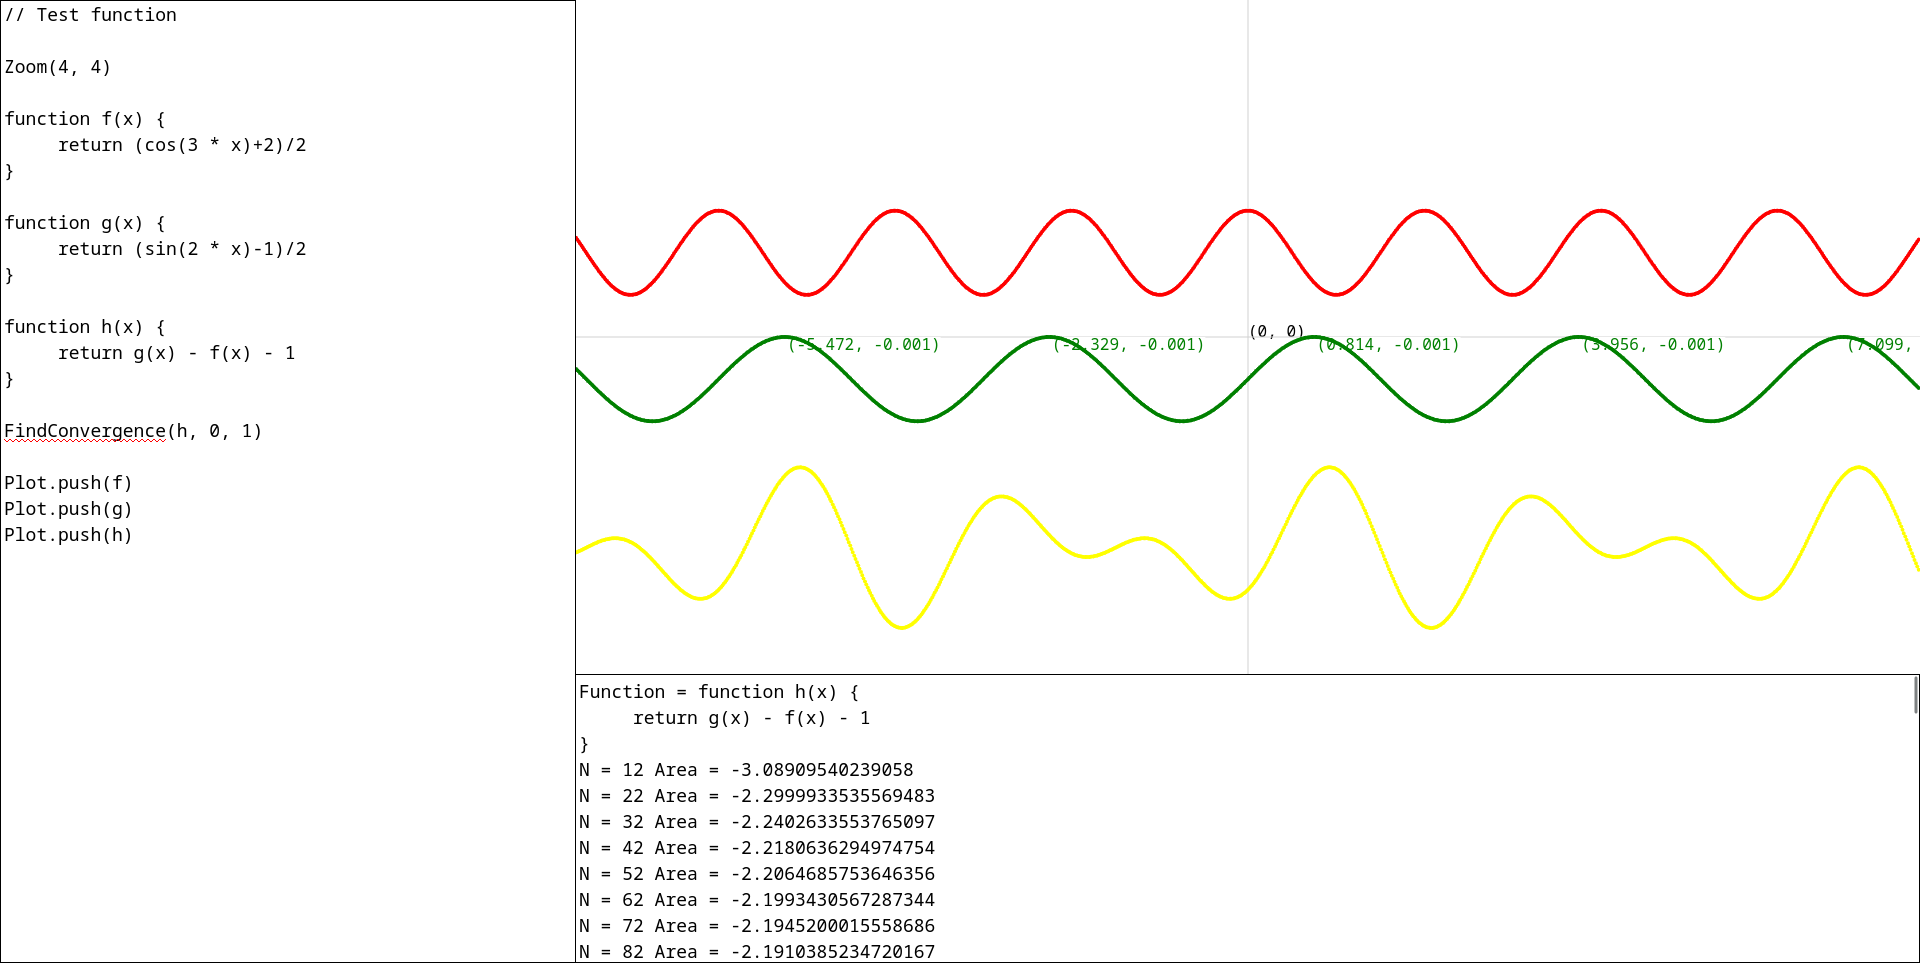
\includegraphics[width=\linewidth]{prototype.png}
	\caption{Integrating and plotting a trigonometric function}
	\label{fig:prototype1}
\end{figure}


\section{Project}

We describe the different parts of the software that we built to implement these numerical methods.

\subsection{Algorithmic approach to numerically solving integrals}

Computing a single integrals is relatively simple. Iteratively we apply trapezoidal or simpson's rule over multiple
samples taken on the function.

\begin{algorithm}
	\caption{Computing an integral of the function $f$.}
	\begin{algorithmic}[1]
		\Procedure{Trapezoidal}{$f_0, f_1$}\Comment{$f_i = f\left(x_i\right)$}
		\State \Return $(f_0 + f_1)/2$
		\EndProcedure
		\Statex
		\Procedure{Integrate}{$s \text{: start}, e \text{: end}, f \text{: function}, n \text{: samples}$}
		\State $h \gets (e - s) / n$
		\State $a \gets 0$\Comment{area under the curve}
		\For{$x \gets s \text{\bf{ to }} e - h \text{\bf{ step }} h$}
		\State $a \gets a + h \cdot Trapezoidal(f(x), f(x + h))$
		\EndFor
		\State \Return $a$
		\EndProcedure
	\end{algorithmic}
\end{algorithm}

To extend this integral to multiple variables we perform integrals on each axis at a time. Implementation of this method
algorithmically requires us to treat inner integrals as functions which we can integrate normally.

$$ g(x) = \int_a^b f(x, y) dy $$

This means that each inner integrals has access the current state of the variables of the outer integrals. We developed
the idea of a `context' which holds values of all previously occuring integrals. In this algorithm we express this with
the function $f^*(x)$ which essentially means that this function not only operates on variable $x$ but also has access
to all other previous variables (now treated as constants).

$$ f^*_i(x) = f(x_0, x_1, ..., x_{i-1}, x)$$

Describing this as a algorithm turns the functions assuming each integrals described from outermost ($0_{th}$) to innermost ($n_{th}$) and the 
these integrals operate in order variables from $x_0$ to $x_n$. This does not need to be case and indeed in our implementation we avoid this
positional lockin by utilizing associative arrays for the arguments of the function instead of positional arguments. However that does not affect
the way the algorithm oprates,

\begin{algorithm}
	\caption{Computing multiple integrals of the function $f$.}
	\begin{algorithmic}[1]
		\Procedure{Multi-Integral}{$l \equiv [(s, e)], f, d, c$}
		\Statex{$l$ are the limits, $f$ is the function to be integrated}
		\Statex{$d$ depth of recursion, $c$ reffers to the variable contexts}
		\If{$| l | = 0$}\Comment{We do not have any more integrals}
		\State \Return $f^*_n(x_n)$ \Comment{$x_i$ are accessed through the `context' variable $c$}
		\Else
		\State $h \gets (l_d.e - l_d.s) / n$
		\State $a \gets 0$\Comment{area under the curve}
		\For{$x_d \gets l_d.s \text{\bf{ to }} l_d.e - h \text{\bf{ step }} h$}

		\State $\text{add\_context\_variable}\left( c, x_d \right)$
		\State $r_0 \gets \text{Multi-Integral}(l, f, d + 1, c)$\Comment{inner integrals as functions}
		\State $r_1 \gets \text{Multi-Integral}(l, f, d + 1, c)$
		\State $\text{remove\_context\_variable}\left( c, x_d \right)$
		\State $a \gets a + h \cdot (r_0 + r_1) / 2$\Comment{Trapezoidal rule}
		\EndFor
		\State \Return $a$
		\EndIf
		\EndProcedure
	\end{algorithmic}
\end{algorithm}

\subsection{Console Interface}

The graphical user interface of the prototype was discarded in favour of a very simple console interface to improve portability of
the software. To provide quality of life features we utilize a console input library Crossline\cite{ac}

A part of the user input also involved accepting a C source file which contained all the function expressions. This file is used to allow runtime
expression changing which is further discussed in the later sections.

The users interact with internal integrator using simple commands like `integrate' and `plot'. Commands like `list' and `pointer' were added to 
aid with debugging perposes.

A special set of macros were developed to allow the `list' function to work and to allow a simple way to return vector values.

\subsection{Runtime expression change}

A major problem with our integrator was the slow execution times of a interpreted language. Since each function
had to be executed multiple times the cost of interpreting added up extremely quickly. We noticed this problem in
the prototype, the website would sometimes stop responding due to the high integrator execution times.

To address this problem it was nessesary to compile the expression down to a native binaries which would run orders
of magnitude faster. To achieve this we utilized the very small c99 complient `tiny c compiler'\cite{ab}.
We spawned a process with the tcc binaries and compiled the expression C file into a Dynamic link library (or Shared Object).
The generated executable is a Position Independent (reffered to as PIE from here). This allowed use to load this executable at runtime
and execute the native binary version of the expressions. An important factor which allowed this was that all the expressions did not have
any side effects i.e. they did not affect memory of the main process. This meant that we did not have to deal with a situation where the
structure of the code changed but the memory held in the process did not leading to fatal memory corruptions or undefined accesses of memory
locations.

We also considered developing a simple scripting language, but that idea was found to be largly out of the scope of this project.

Some of the hurdles we faced while using the tcc compiler included the lack of support for complex data types which is standard for any c11 compilent
compiler like gcc. We had to implement our own version of complex data type.

\subsection{Multiple Integration}

Functionally Multiple Integrals operate similarly to single integrals as demostrated in previous sections. The way we deal with this in our software is
we have a C structure which represents any given integrals with its limits and the variable it is operating on. We can construct a linked list of such integrals
resolving the limits of each integral from outer outer most to inner most. Then integrating the function from inner to to outer integrals. We also incorportate
a special integral computation module which would allow us to compute integrals of common functions which are known not to behave well under simpsons and 
trapezoidal rule of integration.

\subsection{Plotting of Functions}

Each vector valued function is assumed to be of the form $f:\mathbb{R}^2 \rightarrow \mathbb{R}$ This assumption allows us to plot any given 2d or 1d function.

Values for multiple points are sampled from the function. A group of 3 adjescent points are selected a triangle is formed. In this manner a contiguous mesh of
triangles is generated. each triangle is shaded on the basis of their normal values. The shading gives a sense of depth to the plot. Each point is recomputed each
turn of the plot. To achieve higher resolution plot the number of points sampled is increased.

The triangles are displayed on the screen using the cross platform graphics library Raylib\cite{ad}. Raylib allows a streamlined interfacing with accelerated graphics
hardware using the OpenGL API and a simple way to accept user keyboard input.

\subsection{Special Functions}

Some functions like the gamma function do not behave well with generalized integral computation methods, thus special
methods have been developed to specifically deal with these functions. Currently the only function that has been implemented
under this module is the Gamma function. We utilize the Lanczos Aproximation\cite{aa} for the gamma function to compute their values at 
a resonably high speed and acuracy.

\subsection{Examples of Function Integration and Plotting}

\subsubsection{Integrating $sin(x)$ function from 0 to $\pi$\textsuperscript{\ref{fig:example1}}}

\begin{flushleft}
Expression C file to integrate sin function from 0 to $\pi$,
\end{flushleft}

\begin{lstlisting}
#include "function.h"

FUNCTION ( X )
vec_t function(vec_t v)
{
	RETURN_VEC ( sin(v.it[0]) );
}

FUNCTION ( )
vec_t limit_start(vec_t v)
{
	RETURN_VEC ( 0 );
}

FUNCTION ( )
vec_t limit_end(vec_t v)
{
	RETURN_VEC( PI );
}
\end{lstlisting}

\begin{flushleft}
Integrating on variable X from 0 to 3.141593.
\end{flushleft}

\begin{table}[h]
	\centering
	\begin{tabular}{ |c c c c c c| }
		\hline
		\hline
		Step & Variable & $h$ & Start & End & Result \\
		\hline
		\hline
		1 & x & 0.031416 & 0.000000 & 3.141593 & 1.999507 \\
		\hline
		2 & x & 0.030800 & 0.000000 & 3.141593 & 1.999526 \\
		\hline
		3 & x & 0.030208 & 0.000000 & 3.141593 & 1.999544 \\
		\hline
		4 & x & 0.029638 & 0.000000 & 3.141593 & 1.999561 \\
		\hline
		5 & x & 0.029089 & 0.000000 & 3.141593 & 2.000000 \\
		\hline
		6 & x & 0.028560 & 0.000000 & 3.141593 & 2.000000 \\
		\hline
		\hline
	\end{tabular}
\end{table}

\subsubsection{Integrating $sin(x) + sin(y)$ function\textsuperscript{\ref{fig:example2}}}

\begin{flushleft}
Expression C file to integrate $sin(x) + sin(y)$ under the triangle with vertices $(0, 0) (1, 0) (1, 1)$
\end{flushleft}

\begin{lstlisting}
#include "function.h"

FUNCTION  ( X, Y )
vec_t function(vec_t v)
{
	RETURN_VEC ( sin(v.it[0]) + sin(v.it[1]) );
}

FUNCTION ( )
vec_t limit_start_outer (vec_t v)
{
       	RETURN_VEC ( 0 );
}

FUNCTION ( )
vec_t limit_end_outer  (vec_t v)
{
	RETURN_VEC ( 1 );
}

FUNCTION ( )
vec_t limit_start_inner(vec_t v)
{
	RETURN_VEC ( 0 );
}

FUNCTION ( Y )
vec_t limit_end_inner  (vec_t v)
{
	RETURN_VEC ( v.it[0] );
}
\end{lstlisting}

\begin{flushleft}
	Integrating on variable Y then on the inner variable X under the trianglular region with verticles $(0, 0) (1, 0) (1, 1)$
\end{flushleft}

\begin{table}[H]
	\centering
	\begin{tabular}{ | c c c c c c | }
		\hline
		\hline
		Step & Variable & $h$ & Start & End & Result \\
		\hline
		\hline
		1    & x & 0.000000 & 0.000000 & 0.000167 & 0.000000 \\
		\hline
		2    & x & 0.000000 & 0.000000 & 0.000333 & 0.000000 \\
		\hline
		3    & x & 0.000000 & 0.000000 & 0.000500 & 0.000000 \\
		\hline
		4    & x & 0.000001 & 0.000000 & 0.000667 & 0.000001 \\
		\hline
		5    & x & 0.000001 & 0.000000 & 0.000833 & 0.000001 \\
		\hline
		\multicolumn{6}{|c|}{...} \\
		\hline
		n+1  & x & 0.001000 & 0.000000 & 0.999500 & 1.300057 \\
		\hline
		n+2  & x & 0.001000 & 0.000000 & 0.999667 & 1.302110 \\
		\hline
		n+3  & x & 0.001000 & 0.000000 & 0.999833 & 1.302481 \\
		\hline
		n+4  & x & 0.001000 & 0.000000 & 1.000000 & 1.301169 \\
		\hline
		n+5  & y & 0.001000 & 0.000000 & 1.000000 & 0.459997 \\
		\hline
		\hline
	\end{tabular}
\end{table}

\begin{figure}
	\centering
	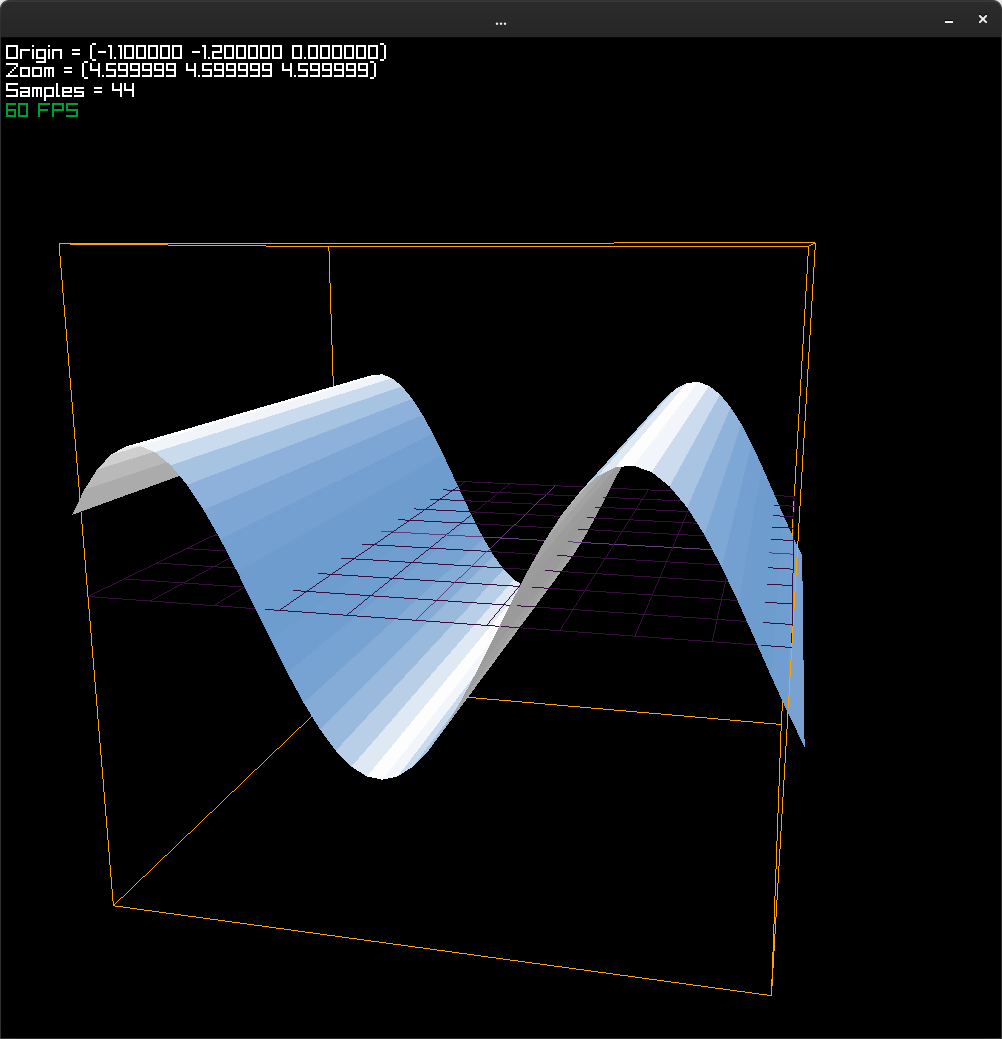
\includegraphics[width=0.65\textwidth]{example1.png}
	\caption{$sin(x)$}
	\label{fig:example1}
\end{figure}

\begin{figure}
	\centering
	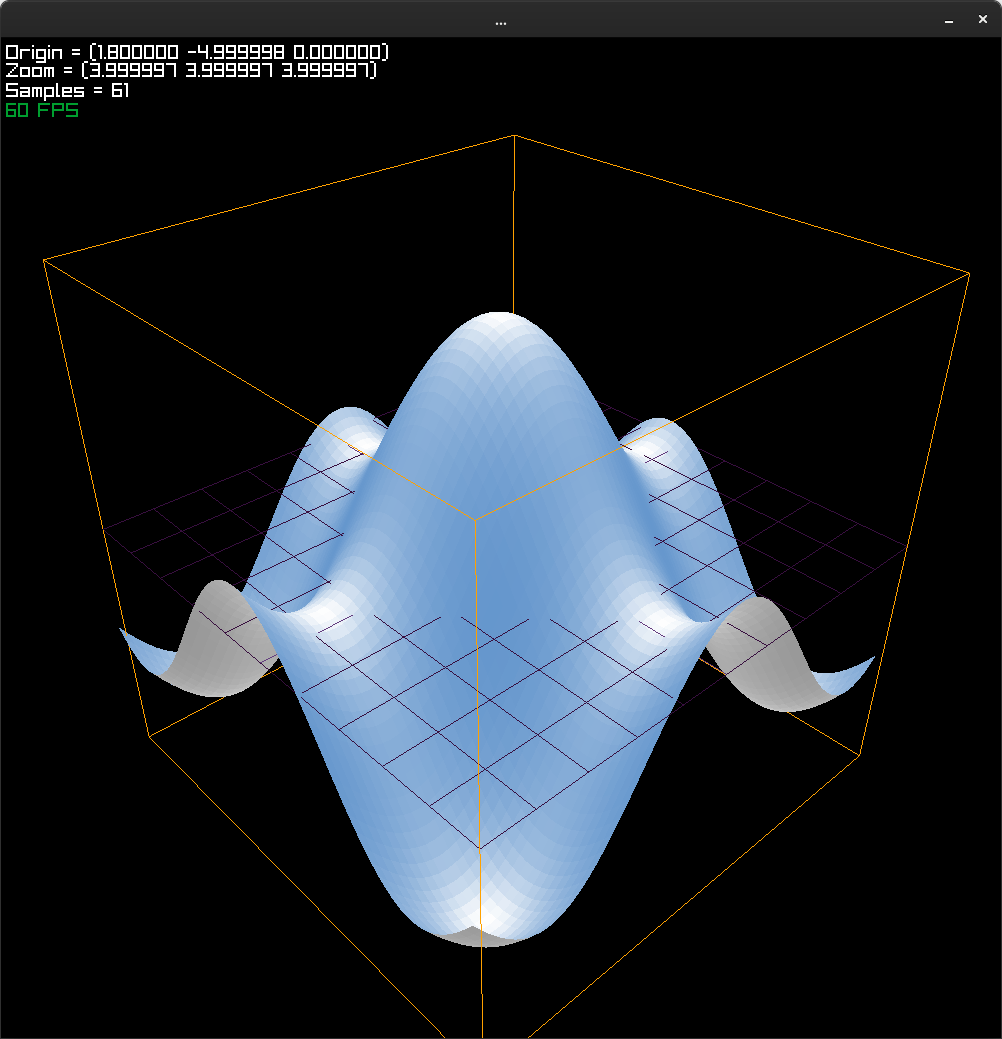
\includegraphics[width=0.65\textwidth]{example2.png}
	\caption{$sin(x) + sin(y)$}
	\label{fig:example2}
\end{figure}

\pagebreak
\section{Results}
\subsection{Gamma function and methods of computing it numerically} 

The gamma function can be defined as,

\begin{align*}
	\Gamma(z) &= \frac{1}{z} \prod_{n = 1}^{\infty} \left[ \frac{1}{1 + \frac{z}{n}} \left(1 + \frac{1}{n} \right)^{z} \right]\\
	\\
	&= \int_0^\infty t^{z-1} e^{-t} dt\\
	\\
	&= z \Gamma(z - 1)
\end{align*}
\\
The gamma function is an relatively difficult function to compute with these simple numerical methods from
a complexity perspective. The major reasons for this being the case are:
\begin{itemize}
	\item The gamma function is computed through an improper integrals.
	\item The function grows at the rate of $O(n!)$ which is very difficult to manage, and precompute.
	\item The function also has discontinuities at the $-ve$ integers
\end{itemize}

To understand the limitations of the program we try to compute and plot the values of the gamma function using
various methods implemented under the plotting and runtime expression compilation tooling we have built.

In the following sections we describe algorithms that have been used to compute the gamma functions. We also
measured the time for computation required to execute these algorithms when implemented under the constraints
of the software we have built. We utilize the implementation of gamma function in pythons math libraries 
to estimate the precision of each method.

\begin{algorithm}
	\caption{Iterated Product method of computing the gamma function}
	\begin{algorithmic}[1]
	\Procedure{Gamma}{$z$}
	\State $g \gets 1 / z$
	\For{$n \gets 1 \text{ \bf{to} } 10^7$}
	\State $a \gets 1 / (1 + z/n)$
	\State $b \gets (1 + 1/n)^z$
	\State $g \gets a \cdot b \cdot g$
	\EndFor
	\State \Return $g$
	\EndProcedure
	\end{algorithmic}
\end{algorithm}

The Algorithm describing the integral solving method has been presented in section 4.1
The "Lanczos Implementation of the Gamma Function" has been described in the paper \cite{aa}.

\pagebreak
\subsection{Comparisn of Compute times of each method of computing Gamma Function}

We perform the gamma function a small sample set of input, and time that operation. This excercise gives us a good idea on the performace of each algorithm
on real hardware. This important because the time complexity of each method is $O(n)$.
\\

\begin{bf}
	\flushleft
	Compute times for the Gamma Function using the infinite product definition.
\end{bf}

\begin{itemize}
	\item Total Time of execution = 7.4433441162109375 seconds
	\item Time of execution for each input = 0.9304180145263672 seconds
\end{itemize}

\begin{table}[H]
	\centering
	\begin{tabular}{ | c c c c | }
		\hline
		\hline
		Input & Output & Actual & Error\\
		\hline
		\hline
		0.1 & 9.513508 & 9.513507698668732 & 3.0133126749376515e-07\\
		\hline
		0.2 & 4.590844 & 4.5908437119988035 & 2.8800119622474085e-07\\
		\hline
		0.3 & 2.991569 & 2.991568987687591 & 1.2312409314318984e-08\\
		\hline
		0.4 & 2.21816 & 2.2181595437576878 & 4.562423123743997e-07\\
		\hline
		2 & 1.0 & 1.0 & 0.0\\
		\hline
		3 & 1.999999 & 2.0 & -9.999999999177334e-07\\
		\hline
		4 & 5.999996 & 6.0 & -3.9999999996709334e-06\\
		\hline
		5 & 23.999976 & 24.0 & -2.3999999999801958e-05\\
		\hline
		\hline
	\end{tabular}
\end{table}

\begin{bf}
	\flushleft
	Compute times for the Gamma Function using the Euler integral definition.
\end{bf}

\begin{itemize}
	\item Total Time of execution = 9.676705837249756 seconds
	\item Time of execution for each input = 1.2095882296562195 seconds
\end{itemize}

\begin{table}[H]
	\centering
	\begin{tabular}{ | c c c c | }
		\hline
		\hline
		Input & Output & Actual & Error\\
		\hline
		\hline
		0.1 & 5.625076 & 9.513507698668732 & -3.8884316986687324\\
		\hline
		0.2 & 3.857274 & 4.5908437119988035 & -0.7335697119988036\\
		\hline
		0.3 & 2.811185 & 2.991568987687591 & -0.18038398768759079\\
		\hline
		0.4 & 2.167838 & 2.2181595437576878 & -0.0503215437576876\\
		\hline
		2 & 0.999988 & 1.0 & -1.2000000000012001e-05\\
		\hline
		3 & 2.0 & 2.0 & 0.0\\
		\hline
		4 & 6.0 & 6.0 & 0.0\\
		\hline
		5 & 24.0 & 24.0 & 0.0\\
		\hline
		\hline
	\end{tabular}
\end{table}

\begin{bf}
	\flushleft
	Compute times for the Gamma Function using the Laconzs aproxmiation.
\end{bf}

\begin{itemize}
	\item Total Time of execution = 0.01519465446472168 seconds
	\item Time of execution for each input = 0.00189933180809021 seconds
\end{itemize}

\begin{table}[H]
	\centering
	\begin{tabular}{ | c c c c | }
		\hline
		\hline
		Input & Output & Actual & Error\\
		\hline
		\hline
		0.1 & 9.513508 & 9.513507698668732 & 3.0133126749376515e-07\\
		\hline
		0.2 & 4.590844 & 4.5908437119988035 & 2.8800119622474085e-07\\
		\hline
		0.3 & 2.991569 & 2.991568987687591 & 1.2312409314318984e-08\\
		\hline
		0.4 & 2.21816 & 2.2181595437576878 & 4.562423123743997e-07\\
		\hline
		2 & 1.0 & 1.0 & 0.0\\
		\hline
		3 & 2.0 & 2.0 & 0.0\\
		\hline
		4 & 6.0 & 6.0 & 0.0\\
		\hline
		5 & 24.0 & 24.0 & 0.0\\
		\hline
		\hline
	\end{tabular}
\end{table}

\subsection{Comparisn of Error of each method of computing Gamma Function}

\begin{figure}[H]
	\centering
	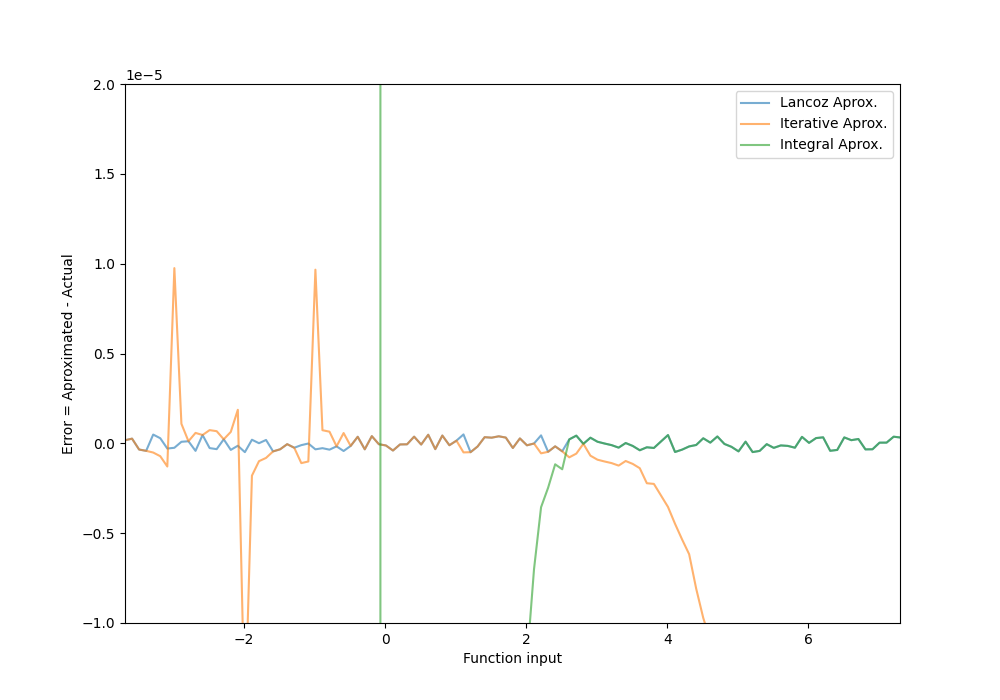
\includegraphics[width=\textwidth]{test.png}
	\label{fig:test}
\end{figure}

From this plot and the previous execution times recorded we can understand that the Lanczos aproximation performs best in all regards.
The integral method performs well for posetive real numbers greater than 2 but fails rapidly for the rest. The iterative method performs
well for real numbers less than 2 and starts to fail rapidly for the rest. However the error is not extremely high given the number only 
deviates at the order of $10^-5$.

\pagebreak
\section{Conclusion}

Simpsons method and trapezoidal methods provide good numerical aproximations for most situations but it may be nessesary to develop specialized
methods in cases where they start to fail. The major points of faliure has been the rapid increase in the limits. The methods outlined perform
well in situtation where the $h$ value is relatively small, but having a very small $h$ is highly impractical since it increases the iteration
count rapidly.

\section{References}
\begin{thebibliography}{2}
	\bibitem{aa} Godfrey, Paul (2001). "Lanczos Implementation of the Gamma Function" \url{http://www.numericana.com/answer/info/godfrey.htm}
	\bibitem{ab} Bellard, Fabrice (2018). "Tiny C Compiler" \url{https://bellard.org/tcc/}.
	\bibitem{ac} Wang, JC (2023). "Crossline" "A small, self-contained, zero-config, MIT licensed, cross-platform, readline and libedit replacement." \url{https://github.com/JunchuanWang80/crossline}.
	\bibitem{ad} Santamaria, Ramon (2025). "Raylib" "A simple and easy-to-use library to enjoy videogames programming" \url{httsp://www.raylib.com}
\end{thebibliography}

\begin{flushleft}
	\begin{bf}
		\large
		Source Code for the project
	\end{bf}
	\begin{itemize}
		\item[-] Integrator Prototype : \url{https://nimcompoo-04.github.io/numlysis/}
		\item[-] Numerical Analysis Integrator : \url{https://www.github.com/NimComPoo-04/NumericalAnalysis}
	\end{itemize}
\end{flushleft}

\end{document}
